% -*- TeX:UTF-8 -*-
%%
%% KAIST 학위논문양식 LaTeX용 (ver 0.4) 예시
%%
%% @version 0.4.1
%% @author  채승병 Chae,Seungbyung (mailto:chess@kaist.ac.kr)
%% @date    2004. 11. 12.
%% @modifier 신호철 (mailto:h.c.shin@kaist.ac.kr)
%% @moddate 2018. 11. 29
%%
%% @requirement
%% teTeX, fpTeX, teTeX 등의 LaTeX2e 배포판
%% + 은광희 님의 HLaTeX 0.991 이상 버젼 또는 홍석호 님의 HPACK 1.0
%% : 설치에 대한 자세한 정보는 http://www.ktug.or.kr을 참조바랍니다.
%%
%% @note
%% 기존에 널리 쓰여오던 차재춘 님의 학위논문양식 클래스 파일의 형식을
%% 따르지 않고 전면적으로 다시 작성하였습니다. 논문 정보 입력부분에서
%% 과거 양식과 다른 부분이 많으니 아래 예시에 맞춰 바꿔주십시오.
%%
%%
%% @acknowledgement
%% 본 예시 논문은 물리학과 박사과정 김용현 님의 호의로 제공되었습니다.
%%
%% -------------------------------------------------------------------
%% @information
%% 이 예제 파일은 hangul-ucs를 사용합니다. UTF-8 입력 인코딩으로
%% 작성되었습니다. hlatex의 hfont는 이용하지 않습니다. --2006/02/11
%% 본 템플릿은 전산학부 김민혁 교수에의해서 버그 수정되었습니다. -- 2016/11/25
%% 전자과 신호철에 의해서 포맷 수정됨 (주로 draft 버전에서의 논문 표시양식)

% @class kaist.cls
% @options [default: doctor, korean, final]
% - doctor: 박사과정 | master : 석사과정
% - korean: 한글논문 | english: 영문논문
% - final : 최종판   | draft  : 시험판
% - pdfdoc : 선택하지 않으면 북마크와 colorlink를 만들지 않습니다.

%indicator for the final version
%N.B. Use \finaltrue for dissertation publication, and use \finalfalse for the proposal and defense
\newif\iffinal
%\finaltrue %to set final marker as true -> final
\finalfalse %set final marker as false -> draft

\iffinal
	\documentclass[doctor,english,final,pdfdoc]{kaist-ucs-improved}
	\usepackage{lmodern} %This suppresses font size warnings in final version
\else
	\documentclass[doctor,english,draft,pdfdoc]{kaist-ucs-improved}
\fi

%Enable numbering upto subsubsection
%Increase the number to enable numbering for lower levels: e.g. \paragraph and \subparagraph
\setcounter{secnumdepth}{3}

% If you want make pdf document (include bookmark, colorlink)
%\documentclass[doctor,english,final,pdfdoc]{kaist-ucs}

% kaist.cls 에서는 기본으로 dhucs, ifpdf, graphicx 패키지가 로드됩니다.
% 추가로 필요한 패키지가 있다면 주석을 풀고 적어넣으십시오,
%\usepackage{...}

% @command title 논문 제목(title of thesis)
% @options [default: (none)]
% - korean: 한글제목(korean title) | english: 영문제목(english title)
\title[korean] {한글 제목}
\title[english]{English title of the dissertation}

% @note 표지에 출력되는 제목을 강제로 줄바꿈하려면 \linebreak 을 삽입.
%       \\ 나 \newline 등을 사용하면 안됩니다. (아래는 예시)
%
%\title[korean]{탄소 나노튜브의 물리적 특성에 대한\linebreak 이론 연구}
%\title[english]{Theoretical study on physical properties of\linebreak
%                carbon nanotubes}
%
% If you want to begin a new line in cover, use \linebreak .
% See examples above.
%


% @command author 저자 이름
% @param   family_name, given_name 성, 이름을 구분해서 입력
% @options [default: (none)]
% - korean: 한글이름 | chinese: 한문이름 | english: 영문이름
% 한문 이름이 없다면 빈 칸으로 두셔도 됩니다.
%
%
% If you are a foreigner , write your name in korean or your korean name.
% If you can't write native character, you can make the chinese blank empty 
% Write as follow
% \author[korean]{family name in korean}{given name in korean}
% \author[chinese]{family name in your native language}{given name in your native language}
% \author[english]{family name in english}{given name in english}
%
\author[korean]{홍}{길 동}
\author[korean2]{홍}{길동}    %이름을 붙여 써 주시기 바랍니다.
\author[chinese]{}{} %Don't want hanja
\author[english]{Hong}{Gildong}

% @command advisor 지도교수 이름 (복수가능)
% @usage   \advisor[options]{...한글이름...}{...영문이름...}{signed|nosign}
% @options [default: major]
% - major: 주 지도교수  | coopr: 공동 지도교수
\advisor[major]{갑}{Gab}{signed}
\advisor[major2]{갑}{Gab}{signed} %한글 성과 한글 이름을 모두 붙여 써 주시기 바랍니다.

%For final draft
\advisorinfo{Professor of Electrical Engineering} %제출승인서에 들어가는 교수님 정보, advisor's information   
%\advisor[coopr]{홍 길 동}{Gil-Dong Hong}{nosign}
%\advisor[coopr2]{홍길동}{Gil-Dong Hong}{nosign}    %한글 성과 한글 이름을 모두 붙여 써 주시기 바랍니다.
%
% 지도교수 한글이름은 입력하지 않아도 됩니다.
% You may not input advisor's korean name
% like this \advisor[major]{}{Chang, Kee Joo}{signed}
%


% @command department {학과이름}{학위종류} - 아래 규칙에 따라 코드를 입력
% @command department {department code}{degree field}
%
% department code
% 2. 석박사학위논문 작성 및 제출요령 4쪽 ~ 5쪽 참고
% 또는 kaist-ucs.cls 의 % @command department 참고

% science: 이학 | engineering: 공학 | business : 경영학
% 박사논문의 경우는 학위종류를 입력하지 않아도 됩니다.
% If you write Ph.D. dissertation, you cannot input degree field.
% The third parameter : a | b | c
% a: 소속된 학과만 쓰는 옵션 (학과에만 소속되어 있는 경우에는 무조건 a를 선택해야 함)
% b: 학과 아래의, 프로그램이나 학제전공에 소속되어 있을 경우에 학과와 프로그램을 함께 쓰는 옵션
% c: 학과 아래의, 프로그램이나 학제전공에 소속되어 있을 경우에 학과를 쓰지 않고 프로그램이나 학제전공의 이름만 쓰는 옵션 
% 
% a: it represents only the name of department. (if you aren't in the program under the department, must choose a)
% b: it represents the names of department and the program that is under the department (consider this when you are in the program not only department)
% c: it represents only the name of program that is under the department (consider this when you are in the program not only department)

\department{EE}{engineering}{a}

% @command studentid 학번(ID)
\studentid{20155185}

% @command referee 심사위원 (석사과정 3인, 박사과정 5인)
\referee[1]{갑}
\referee[2]{을}
\referee[3]{병}
\referee[4]{정}
\referee[5]{무}
% \referee[5] {Barack Obama}
% Of course english name is available

% @command approvaldate 지도교수논문승인일
% @param   year,month,day 연,월,일 순으로 입력
\approvaldate{2020}{11}{30} %SHOULD BE MODIFIED
\fontsize{17.28pt}{17.28pt}\selectfont %Font size changed from 18pt to 17.28pt to remove warnings

% @command refereedate 심사위원논문심사일
% @param   year,month,day 연,월,일 순으로 입력
\refereedate{2020}{11}{30} %SHOULD BE MODIFIED

% @command gradyear 졸업년도
\gradyear{2020} %SHOULD BE MODIFIED

% 본문 시작
\begin{document}
    % 앞표지, 속표지, 학위논문 제출승인서, 학위논문 심사완료 검인서는
    % 클래스 옵션을 final로 지정해주면 자동으로 생성되며,
    % 반대로 옵션을 draft로 지정해주면 생성되지 않습니다.
    % 학위논문 제출 승인서에서 자신의 전공과 교수님의 정보를 바꾸기 위해서는 첨부되어있는 제목이 kaist-ucs인 class 문서에 들어가서 ####################로 표시  
    % 한 부분을 바꾸시길 바랍니다.

    % 논문 서지, 초록, 핵심 낱말, 영문 초록, 영어 핵심 낱말 (Information of thesis, abstract in korean, keywords in korean, abstract in english, keywords in english)
    %% 한글 초록은 500자를, 영문 초록은 300 낱말을 넘지 않아야 함
    %% 핵심 낱말은 5 개 이내로 넣음
    %% 한글 초록에 영문 글자를 쓰지 않도록 한다.
		\thesisinfo
   
    %\begin{summary}      
    %지난 10여 년간 탄소 나노튜브는 자체의 독특한 전기적, 기계적 성질로
    %인하여 다가오는 나노기술 분야의 이상적인 기초물질중의 하나로 떠오르고
    %있다. 흑연을 감는 세세한 방법에 따라 전기적 특성이 금속성에서 1eV의
    %띠간격을 가지는 반도체 특성까지 다양한 분포로 존재한다.
    %본 학위논문에서는 탄소 나노튜브의 여러 물리적 성질에 대해 고찰하는데,
    %기본적으로 제일원리 밀도함수 이론과 밀접결합근사 모형을 사용하여 전기적
    %특성과 그 제어 방법, 자기적 특성, 그리고 수송특성 등을 다루고자 한다.
    %\end{summary}
   
    %\begin{Korkeyword}
    % 가, 나, 다
    %\end{Korkeyword}

		%Locate abstract in a separate file
		% ABSTRACT
\begin{abstract}
	Input dissertation abstract here.
\end{abstract} 

% KEYWORD
\begin{Engkeyword}
	keyword1, keyword2, keyword3
\end{Engkeyword}


    \addtocounter{pagemarker}{1}                 % 백색별지분을 고려
    \newpage  
  
		\iffinal
			% 목차 (Table of Contents) 생성
			\tableofcontents

			% 표목차 (List of Tables) 생성
			\listoftables

			% 그림목차 (List of Figures) 생성
			\listoffigures
		\else
			\label{paperlastromanpagelabel} %For removing warning in draft mode
			\pagenumbering{arabic} % Draft mode has no pagenumbering so add it.
		\fi

    % 위의 세 종류의 목차는 한꺼번에 다음 명령으로 생성할 수도 있습니다.
    %\makecontents
%% 한글로 쓴 논문에는 본문에 영문 글자를 쓰지 않는다. 다만, 꼭 필요할 때에는 ‘한글 낱말 (영문 낱말)’ 꼴로 적는다.
%% 이하의 본문은 LaTeX 표준 클래스 report 양식에 준하여 작성하시면 됩니다.
%% 하지만 part는 사용하지 못하도록 제거하였으므로, chapter가 문서 내의
%% 최상위 분류 단위가 됩니다.
%% You cannot use 'part'

		%Chapters in separate files
		\chapter*{Introduction} %Don't want chapter number for intro
Put dissertation introduction here.
Test citation~\cite{dean2011characterization}

\section{Blah}
\subsection{Blah}
\subsubsection{Blah}

		\chapter{Chapter with number}
\section{그림과 표를 본문에서 이야기하기}

본문에서 그림과 표에 관해 이야기를 할 때도 인용에서처럼 하시면 됩니다.

%% Table in a separate file
%%
%% 표 삽입 예시
%% Example. how to insert table
%%
\begin{table}[t]
\caption[캡션제목 넣으십시오]{표 제목을 넣으십시오.
}
\label{mag-tab1}
\begin{center}
\begin{tabular} {ccccccccccc}
\hline\hline
& & BF &\multicolumn{2}{c}{SW-I}&&\multicolumn{2}{c}{SW-II}&SW-III&CAP&\\
\cline{4-5} \cline{7-8}
&               &   &  Para & Ferro &&   Para &  Ferro &      &      &\\
\hline
& $E$ (eV)      & 0 & 7.796 & 7.832 && 10.418 & 10.408 & 11.5 & 13.2 &\\
& $M$ ($\mu_B$) & 0 &     0 &  1.94 &&      0 &   2.06 &    0 &    0 &\\
\hline\hline
\end{tabular}
\end{center}
\end{table}
 %Path viewed from top directory


%%
%% 그림 삽입 예시
%% Example. how to insert graph
%%
%% Note. 가급적 \includegraphics 명령을 사용하십시오.
%% Recommen : Use \includegraphics to insert graph.
%%
\begin{figure}[t]
    \centerline{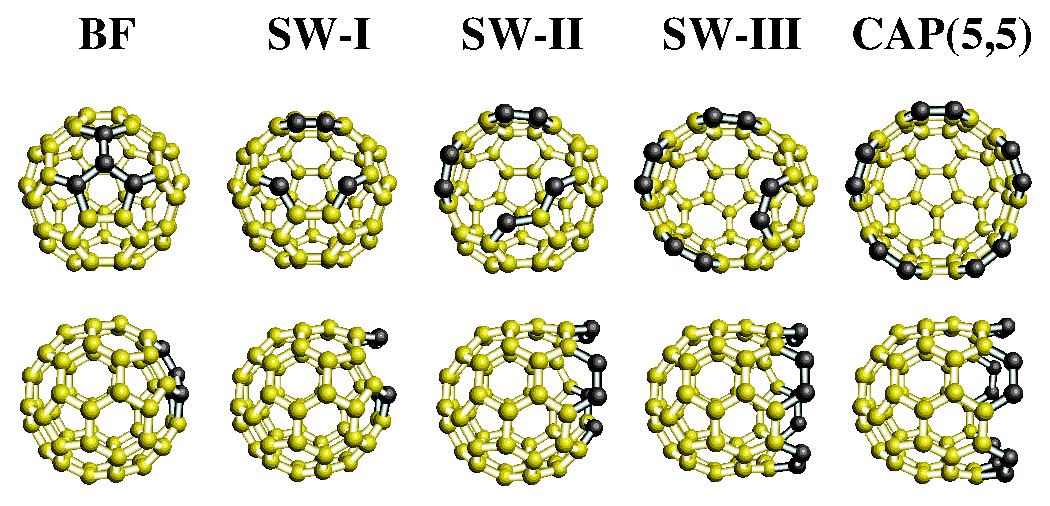
\includegraphics[width=12.5cm]{figures/sample-fig1}} %Path viewed from top directory
    \caption[캡션제목 넣으십시오]{그림 제목을 넣으십시오.
    } \label{mag-fig1}
\end{figure}

		\chapter{Another Numbered Chapter}
\section{Blah}
\subsection{Blah}
\subsubsection{Blah}

		\chapter*{Conclusion} %Don't want chapter number for conclusion
Conclusion comes here.



%%
%% 참고문헌 시작
%% bibliography
%% 위는 보기이므로 학과 또는 논문의 특성에 맞게 조정 가능함. 다만, 참고문헌마다 충분한 정보가 들어 있어야 한다.

%Bibliography
{\footnotesize
	\bibliographystyle{splncs03}
	\bibliography{references/refGeneral}
}

%%
%% 사사 시작
%% Acknowledgement
%% 사사 작성은 선택사항임
% @command acknowledgement 감사의글
% @options [1 | 2 | 3 |4 ]
% - 1 : 본문과 감사의 글이 둘 다 한글일 때  | 2 : 본문은 한글인데 감사의 글이 영어일 때 | 3 :  본문과 감사의 글이 둘 다 영어일 때  | 4 : 본문은 영어인데 감사의 글이 % 한글일 때 

\iffinal
	\acknowledgment[4]
	감사를 드립니다.
\fi

%%
%% 약력 시작
%% Curriculum Vitae
%% 약력 작성은 선택사항임. 약력 내용도 알맞게 바꿀 수 있음
% @command curriculumvitae 이력서
% @options [1 | 2 | 3 |4 ]
% - 1 : 본문과 약력이 둘 다 한글일 때  | 2 : 본문은 한글인데 약력이 영어일 때 | 3 :  본문과 약력이 둘 다 영어일 때  | 4 : 본문은 영어인데 약력이 한글일 때 

\iffinal
	\curriculumvitae[3]
		% @environment personaldata 개인정보
		% @command     name         이름
		%              dateofbirth  생년월일
		%              birthplace   출생지
		%              domicile     본적지
		%              address      주소지
		%              email        E-mail 주소
		% - 위 6개의 기본 필드 중에 이력서에 적고 싶은 정보를 입력
		% input data only you want
		\begin{personaldata}
				\name       {안 진 현}
				\dateofbirth{199x}{x}{xx}
				\birthplace {...}
				\address    { ...}
		 \end{personaldata}

		% @environment education 학력
		% @options [default: (none)] - 수학기간을 입력
		\begin{education}
				\item[2007. 3.\ --\ 2009. 2.] 고등학교 (2년 수료)
				\item[2009. 2.\ --\ 2013. 8.] 한국과학기술원 수리과학과 (학사)
				\item[2013. 9.\ --\ 2016. 2.] 한국과학기술원 수리과학과 (석사)
		\end{education}

		% @environment career 경력
		% @options [default: (none)] - 해당기간을 입력
		\begin{career}
				\item[2013. 9.\ --\ 2016. 2.] 한국과학기술원 수리과학과 일반조교
		\end{career}

		% @environment activity 학회활동
		% @options [default: (none)] - 활동내용을 입력
%%    \begin{activity}
%%        \item J. Choi, \textbf{Yong-Hyun Kim}, K.J. Chang, and D. Tomanek,
%%             \textit{Occurrence of itinerant ferromagnetism in C/BN superlattice
%%             nanotubes}, 5th Asian Workshop on First-Principles Electronic
%%             Structure Calculations, Seoul (Korea), October., 2002.
%%    \end{activity}
%% 학회활동을 쓰고싶으시면, 이 문서와 클래스 문서의 학회활동 부분을 사용하십시오.

		% @environment publication 연구업적
		% @options [default: (none)] - 출판내용을 입력
		\begin{publication}
				\item J. Ahn, \textit{Analysis of Tail Probability of Interference at a Node in 2-dimensional Homogeneous Poisson Point Process}, Master Thesis, Korea Adv. Inst. Science, Techn., Daejeon, Republic of Korea, 2016.
		\end{publication}

\fi

  \label{paperlastpagelabel}     % <-- 추가 부분: 마지막 페이지 위치 지정	
%% 본문 끝
\end{document}
